\begin{titlepage}
	\maketitle
	\tableofcontents
\end{titlepage}

\pagebreak

%\resume

\chapter{Getting Started}
\section{Requirements}

\subsection{Web Browsers}

\par Ext JS 4 supports all major web browsers, from Internet Explorer 6 to the latest version of Google Chrome. During development, however, we recommend that you choose one of the following browsers for the best debugging experience:
\begin{itemize}
\item Google Chrome 10+
\item Apple Safari 5+
\item Mozilla Firefox 4+ with the Firebug Web Development Plugin
\end{itemize}
\par This tutorial assumes you are using the latest version of Google Chrome. If you don't already have Chrome take a moment to install it, and familiarize yourself with the Chrome Developer Tools.\\

\subsection{Open Source License}
\par Sencha is an avid supporter of open source software. The open source license is the appropriate option if you are creating an open source application under a license compatible with the GNU GPL license v3. Although the GPLv3 has many terms, the most important is that you must provide the source code of your application to your users so they can be free to modify your application for their own needs.\\
\subsection{Specific Requirements for Swip}
\par Requirements:
\begin{itemize}
\item Netbeans + Glassfish
\item svn
\item Joseki (ask Camille about installation)
\end{itemize}
   
\section{Installation}

 Installation of the framework into a Netbeans Web project
\begin{itemize}
   \item Download Sencha Extjs  http://www.sencha.com/products/extjs/download/
   \item Unzip and copy to the Netbeans web folder
\end{itemize}
 Installation of the SWIP
\begin{itemize}  
\item You need to have an svn configured.
\item Select Team - Chekout 
\item Repository Url: https://swip.svn.sourceforge.net/svnroot/swip, Repository Folder: Swip
\item You have to start a Joseki server before launching a project
\item Don’t install the Glassfish Web server which goes directly with Netbeans, you need to download the latest version from the internet and to install separately, otherwise the application will not work.
\item To run the application press F6 and it opens in a browser.
\end{itemize}

\chapter{MVC Architecture}
\par Here's how we define MVC-like pattern architecture:
\begin{itemize} 
\item Model is a collection of fields and their data (e.g. a User model with username and password fields). Models know how to persist themselves through the data package, and can be linked to other models through associations. Models are normally used with Stores to present data into grids and other components
\item View is any type of component - grids, trees and panels are all views.
\item Controllers are special places to put all of the code that makes your app work - whether that's rendering views, instantiating Models, or any other app logic.
\end{itemize}
\section{File Structure}
\subsection{General structure} 
\par The following is the recommended directory structure for an Ext JS application:
\begin{itemize}
\item[-] appname
\item[] \begin{itemize}
\item[-] app
       \begin{itemize}
	\item[-] namespace
	\item[]
		\begin{itemize}
	   		\item[-] Class1.js
		   	\item[-] Class2.js
		   	\item[-] ...
		\end{itemize}
	\end{itemize}
\item[-] extjs
\item[-] resources
	\begin{itemize}
	    \item[-]    css
	    \item[-] images
	     \item[-] ...
	\end{itemize}

\item[-] app.js
\item[-] index.html
\end{itemize}
\end{itemize}
\begin{itemize}
\item appname is a directory that contains all your application's source files
\item app contains all your classes
\item extjs contains the Ext JS 4 SDK files
\item resources contains additional CSS and image files which are responsible for the look and feel of the application, as well as other static resources (XML, JSON, etc.)
\item index.html is the entry-point HTML document
\item app.js contains your application's logic
\end{itemize}

\subsection{MVC File Structure}
%\begin{figure}[h]
%\centering
%
\includegraphics[width=200mm]{img/sencha.png}
%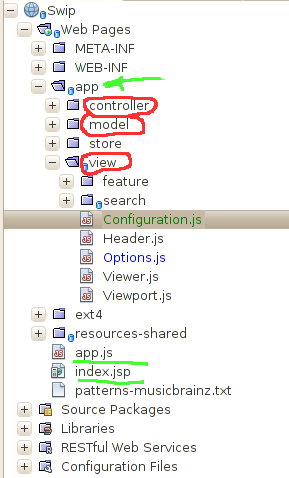
\includegraphics{img/sencha-mvc.png}
%\caption{Swip MVC model}
%\label{fig:sencha-mvc}
%\end{figure}
\par Ext JS 4 applications follow a unified directory structure that is the same for every app. In MVC layout, all classes are placed into the app folder, which in turn contains sub-folders to namespace your models, views, controllers and stores. Here is how the folder structure for the SWIP:
%\ref{fig:sencha-mvc}
\begin{center}
	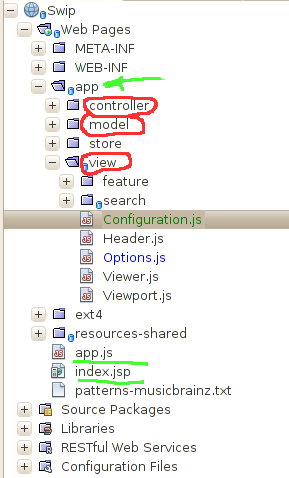
\includegraphics[width=0.75\textwidth]{img/sencha-mvc.png}
	\captionof{figure}{Swip MVC model}
\end{center}
In our application, we are encapsulating the whole application inside standard Netbeans web folder. Essential files from the Ext JS 4 SDK are wrapped inside ext4 folder. In the most of cases an Extjs web application contains a main .html file index.html, however due to specific structure of Netbeans web application we use a .jsp file instead. Hence the content of our index.jsp looks like this: \\
\lstset{
	%backgroundcolor=\color{grey},
	framexleftmargin=5mm, 
	frame=shadowbox, 
	rulesepcolor=\color{blue},
	basicstyle=\small,
	commentstyle=\color{white}, 
	stringstyle=\ttfamily,
	showstringspaces=false,
	postbreak=\space, breakindent=5pt, breaklines
}

\begin{lstlisting}[language=HTML] 
<%@page contentType="text/html" pageEncoding="UTF-8"%>
<!DOCTYPE html>
<html>
  <head>
      <meta http-equiv="Content-Type" content="text/html;charset=UTF-8">
      <title>Swip</title>
      <link rel="stylesheet" type="text/css" href="ext4/resources/css/ext-all.css">
      <link rel="stylesheet" type="text/css" href="resources-shared/css/swip.css">
      <script type="text/javascript" src="ext4/ext-all-debug.js"></script>
      <script type="text/javascript" src="app.js"></script>          
  </head>
  <body>
 </body>
</html>
\end{lstlisting}

\section{Creating the application}
\par Every Ext JS 4 application starts with an instance of Application class. The Application contains global settings for your application (such as the app's name), as well as maintains references to all of the models, views and controllers used by the app. An Application also contains a launch function, which is run automatically when everything is loaded. 
Let's start coding our application. First we need to pick a global namespace for this application. All Ext JS 4 applications should only use a single global variable, with all of the application's classes nested inside it. All of your Application's classes (such as its Models, Views and Controllers) will reside under this single namespace, which drastically lowers the chances of colliding global variables. Usually we want a short global variable so in this case we're going to use "SWIP":\\
\begin{lstlisting}[language=HTML]
Ext.Loader.setConfig({
       enabled : true,
       paths   : {
           Swip : 'web'
       } 
   });
Ext.application({
   name: 'SWIP',
   autoCreateViewport: true,
   paths: {
       'Ext.ux': 'ext4/examples/ux/' 
   },
   
   controllers: [
       'SwipController'
   ]
});
	
\end{lstlisting}


\par There are a few things going on here. First we invoked Ext.application to create a new instance of Application class, to which we passed the name "SWIP". This automatically sets up a global variable SWIP for us, and registers the namespace to Ext.Loader, with the corresponding path of paths option. 
When the page is ready and all of your JavaScript has loaded, your Application's launch function is called, at which time you can run the code that starts your app. Usually this consists of creating a Viewport. We set autoCreateViewport to true to automatically load and instantiate AppName.view.Viewport before firing the launch function. \\

\par Because an Ext.app.Application represents an entire app, we should tell it about the other parts of the app - namely the Models, Views and Controllers that are bundled with the application. Note that we didn't actually list the Views directly in the Application itself. This is because Views are managed by Controllers, so it makes sense to keep those dependencies there.\\ 

\section{Components}
%\begin{figure}[h]
%\centering
%
\includegraphics[width=200mm]{img/sencha.png}
%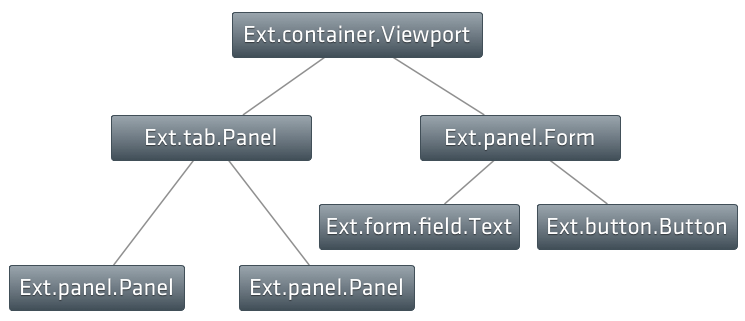
\includegraphics{img/hierarchy.png}
%\caption{Sencha components hierarchy}
%\label{fig:sencha-components}
%\end{figure}
\par An Ext JS application's UI is made up of one or many widgets called Components. All Components are subclasses of the Ext.Component class which allows them to participate in automated lifecycle management including instantiation, rendering, sizing and positioning, and destruction. 
A Container is a special type of Component that can contain other Components. A typical application is made up of many nested Components in a tree-like structure that is referred to as the Component hierarchy.Child Components are added to a Container using the Container's items configuration property.
 A typical application's Component hierarchy starts with a Viewport at the top, which has other Containers and/or Components nested within it:

\begin{center}
	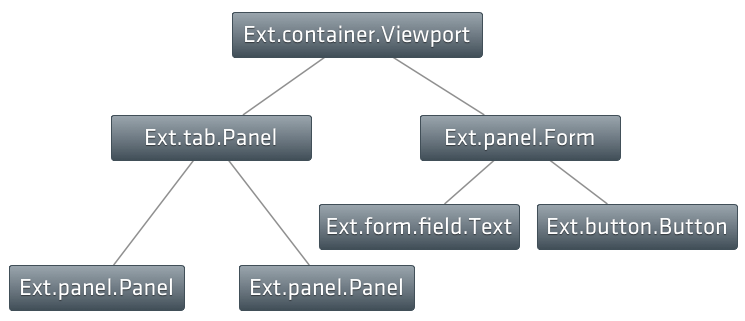
\includegraphics[width=1.00\textwidth]{img/hierarchy.png}
	\captionof{figure}{Sencha components hierarchy}
\end{center}

\begin{center}
	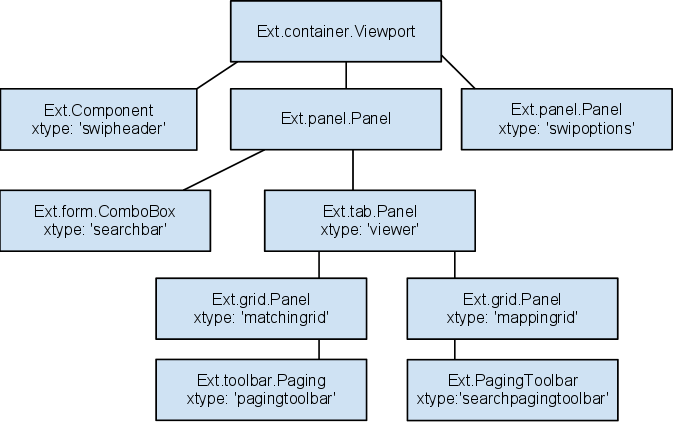
\includegraphics[width=1.00\textwidth]{img/swip_hierarchy.png}
	\captionof{figure}{Swip component hierarchy}
\end{center}

\subsection{XTypes and Lazy Instantiation}
\par Every Component has a symbolic name called an xtype. For example Ext.panel.Panel has an xtype of 'panel'. In a large application, however, not all of the Components need to be instantiated right away, and some Components might never be instantiated depending on how the application is used.This is where xtypes come in handy by allowing a Container's children to be configured up front, but not instantiated until the Container determines it is necessary.
Here we represent a digram of our Application Component hierarchy with the following xtypes.\\
\begin{center}
       \begin{tabular}{ | l | p{10cm} |}
                \hline
		xtype & description \\ \hline
		swipheader & a simple component with the application title \\ \hline
		swipoptions & a panel with accordion layout containing settings and credits \\ \hline
		searchbar & a combobox for the search query input with a local history search in the droplist \\ \hline
		viewer & a tabpanel containing results of the execution such as matchings, mappings and the query represented in Pivot language \\ \hline
		mappingrid & a grid panel containing the mapping results \\ \hline
		matchingrid & a grid panel containing the matching results \\ \hline
		pagingtoolbar & a standard paging toolbar for grid navigation \\ \hline
		searchpagingtoolbar & a custom paging toolbar for grid navigation \\
		\hline
	\end{tabular}
	\captionof{table}{Swip components and their xtypes}
	\label{tab:}
\end{center}
	The below figure illustrates the component hierarchy applied to our case.
\begin{center}
	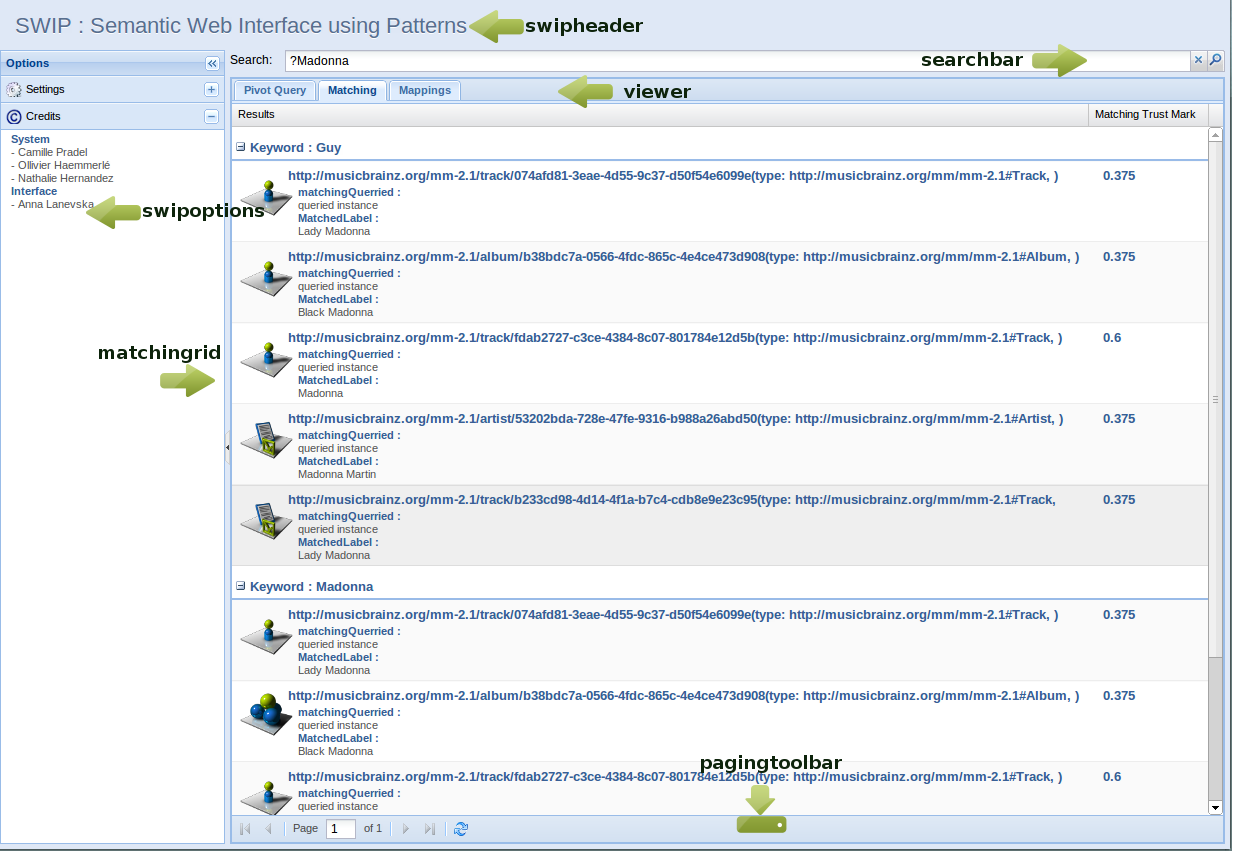
\includegraphics[width=1.00\textwidth]{img/components.png}
	\captionof{figure}{Swip components}
\end{center}

\section{Controller} 
Controllers are the glue that binds an application together. All they really do is listen for events (usually from views) and take some action. Here's how we might create a Controller:
\begin{lstlisting}[language=Java]
var model;
Ext.define('SWIP.controller.SwipController', {
   extend: 'Ext.app.Controller',
   stores: ['Mappings','HistoryRecords','Matchings'],
   models: ['Mapping','HistoryRecord','Matching'],
   views: ['search.Grid', 'search.SearchBar','Viewer','search.MatchingGrid'],
   refs: [{
       ref: 'searchbar',
       selector: 'searchbar'
   },
   {
       ref: 'searchgrid',
       selector: 'searchgrid'
   },
   {
       ref: 'matchingrid',
       selector: 'matchingrid'
   },        
   {
       ref: 'viewer',
       selector: 'viewer'
   }],
   init: function() {
       this.control({
           'searchgrid': {
               itemdblclick: this.viewSearchResult
           },
           'searchbar':{
               render: this.onSearchBarRender,
               afterrender: this.onSearchBarAfterRender,
               change: this.onSearchBarChange,
               trigger1click: this.onSearchBarTrigger1Click, 
               trigger2click: this.onSearchBarTrigger2Click   
           }
       });},
	viewSearchResult: function(grid, record) {
    	var viewer = this.getViewer();
       	Ext.Function.defer(function () {
        	viewer.add({
            	title: record.get('descriptiveSentence'),
               	iconCls: 'tabs-icon',
               	html: record.get('sparqlQuery'),
               	closable: true
           	});
       	}, 100);
   	},
...	
\end{lstlisting}
\par The init function is a special method that is called when your application boots. It is called before the Application's launch function is executed so gives a hook point to run any code before your Viewport is created. The init function is a great place to set up how your controller interacts with the view, and is usually used in conjunction with another Controller function - control. The control function makes it easy to listen to events on your view classes and take some action with a handler function. We use this.control to set up listeners on views in our application. The control function uses the ComponentQuery engine to quickly and easily get references to components on the page.In brief though, it allows us to pass a CSS-like selector that will find every matching component on the page. \\

\subsection{Using refs} 
\par One of the most useful parts of Controllers is the ref system. These use the Ext.ComponentQuery to make it really easy to get references to Views on your page. Let's look at an example of this now: \\
\begin{lstlisting}[language=Java]
refs: [{
       ref: 'searchbar',
       selector: 'searchbar'
   },
   {
       ref: 'searchgrid',
       selector: 'searchgrid'
   },
   {
       ref: 'matchingrid',
       selector: 'matchingrid'
   },  
   {
       ref: 'viewer',
       selector: 'viewer'
   }],
\end{lstlisting}
\par This example assumes the existence of a component of xtype viewer (a tab panel incorporating Mappings, Matchings and Pivot Query). 
In our refs array, we set up a reference to the viewer.There are two parts to this - the 'selector', which is a ComponentQuery selector which finds any viewer on the page and assigns it to the reference 'viewer'. By giving the reference a name, we get a number of things for free. The first is the getViewer function that we use in the  viewSearchResult method above. This is generated automatically by the Controller based on the name of our ref, which was capitalized and prepended with get to go from 'viewer to 'getViewer'. \\
\begin{lstlisting}[language=Java]
viewSearchResult: function(grid, record) {
       var viewer = this.getViewer();
       Ext.Function.defer(function () {
           viewer.add({
               title: record.get('descriptiveSentence'),
               iconCls: 'tabs-icon',
               html: record.get('sparqlQuery'),
               closable: true
           });
       }, 100);},
\end{lstlisting} 
\par The way this works is that the first time getViewer is called by your code, the ComponentQuery selector is run and the first component that matches the selector ('viewer' in this case) will be returned. All future calls to getViewer will use a cached reference to that viewer. Usually it is advised to use a specific ComponentQuery selector that will only match a single View in your application (in the case above our selector will match any viewer on the page). \\
\par Bringing it all together, our init function is called when the application boots, at which time we call this.control to listen to any double click on a item in the searchgrid and call our viewSearchResult function. When the item is doubleclicked we use out getViewer function to add a new tab to the grid. You can create any number of refs and control any number of components this way, simply adding more functions to your Controller as you go. \\
\par Refs aren't the only thing that generate convenient getter methods. Controllers often have to deal with Models and Stores so the framework offers a couple of easy ways to get access to those too. Let's look at another example:\\
\begin{lstlisting}[language=Java]
Ext.define('SWIP.controller.SwipController', {
	extend: 'Ext.app.Controller',
   	stores: ['Mappings','HistoryRecords','Matchings'],
   	models: ['Mapping','HistoryRecord','Matching'],
   	views: ['search.Grid', 'search.SearchBar','Viewer','search.MatchingGrid'],
   	..............................
   	onSearchBarChange: function(){
    	var comboSearchBar = this.getSearchbar();
       	comboSearchBar.store   = this.getHistoryRecordsStore();
       	comboSearchBar.store.load();
   	}
\end{lstlisting}
\par By specifying Models and Stores that the Controller cares about, it again dynamically loads them from the appropriate locations (app/model/HistoryRecord.js, app/store/HistoryRecords.js etc) and creates getter functions for them all. The example above will set a HistoryRecords store as store of the combobox comboSearchBar to implement a local search history. When a user types a character this event updates a drop-down list. 
To create a Model and a Store getter we add a Model() and a Store() endings respectively to their names (ex.: model 'Mapping'-getter getMappingModel()).\\

\section{Models} 
\par The centerpiece of the data package is Ext.data.Model. A Model represents some type of data in an application - for example our application has models for Mapping, Matching and HistoryRecord. A Model represents some object that your application manages. Models are registered via the model manager, and are used by stores, which are in turn used by many of the data-bound components in Ext. Models are defined as a set of fields and any arbitrary methods and properties relevant to the model. For example: \\
\begin{lstlisting}[language=Java]
Ext.define('SWIP.model.Matching', {
   extend   : 'Ext.data.Model',
   fields: [
       {
           name: 'keyWord'
       },  
       {
           name: 'matchingType'
       },
       {
           name: 'uri'
       },
       {
           name: 'matchingQuerried'
       },
       {
           name: 'matchingMatchedLabel'
       },
       {
           name: 'matchingTrustMark'
       } 
   ]});
\end{lstlisting}
\par The fields array is turned into a MixedCollection automatically by the ModelManager, and all other functions and properties are copied to the Model's prototype. Now we can create instances of our HistoryRecord model and call any model logic we defined: \\
\begin{lstlisting}[language=Java]
model = Ext.ModelMgr.create({
               query: value, 
               searchDate: new Date()
           }, 'SWIP.model.HistoryRecord');
\end{lstlisting}

\section{Stores}
\par It is very common to want to load a set of Model instances to be displayed and manipulated in the UI. We do this by creating a Store: \\
\begin{lstlisting}[language=Java]
var store = Ext.create('SWIP.store.HistoryRecords', {
   extend    : 'Ext.data.Store',
   model     : 'SWIP.model.HistoryRecord',
   storeId   : 'HistoryRecords',
   proxy     : {
                  type: 'localstorage',
                  id : 'local-id'
              }
});
//uses the Proxy we set up on Model to load the Store data
store.load();
\end{lstlisting}
\par A Store is just a collection of Model instances - usually loaded from a server somewhere. Store can also maintain a set of added, updated and removed Model instances to be synchronized with the server via the Proxy. The Store class encapsulates a client side cache of Model objects. Stores load data via a Proxy, and also provide functions for sorting, filtering and querying the model instances contained within it. Creating a Store is easy - we just tell it the Model and the Proxy to use to load and save its data:\\
\begin{lstlisting}[language=Java]
Ext.define('SWIP.store.Mappings', {
   extend    : 'Ext.data.Store',
   singleton : true,
   model     : 'SWIP.model.Mapping',
   storeId: 'Mappings',
   autoLoad: false,
   restful: true,
   proxy:  {
       type: 'rest',
       url: 'resources/swip/mappings/{plquery}',    
       headers: {
           'Content-type': 'application/json'
       },
       reader: new Ext.data.JsonReader({
           root:'queryInterpretation',
           totalProperty: 'total'  
       },
       [{
           name: 'sparqlQuery'
       },
       {
           name: 'descriptiveSentence'
       },
       {
           name: 'mappingDescription'
       },
       {
           name: 'relevanceMark'
       } 
       ])
   },
   constructor : function() {
       this.callParent(arguments);
   }                                                                  
 });
\end{lstlisting}
\par In the example above we configured an Rest proxy to load data from the url 'resources/swip/mappings/\{plquery\}'. We told our Proxy to use a JsonReader to parse the response from the server (a JSON file with a root 'queryInterpretation' ) into Model object. \\
\par JSON (Javascript Object Notation) is a text-based, human-readable data interchange format used for representing simple data structures and objects in Web browser-based code. JSON is used in Javascript on the Internet as an alternative to XML for organizing data.\\
\par Sample JSON file: \\
\begin{lstlisting}[language=Java]
{"queryInterpretation":
	[{
		"descriptiveSentence": "some songs from Madonna!?",
		"mappingDescription":"mapping description",
		"relevanceMark":"0.59460354",
		"sparqlQuery": "query"
    },
	{
		"descriptiveSentence":"some songs from ?Madonna of the Wasps?",
		"mappingDescription":"mapping description",
		"relevanceMark":"0.59460354",
		"sparqlQuery":"query2"
	}
]}
\end{lstlisting}

\par It’s analogue in xml: \\

\begin{lstlisting}[language=XML]
<?xml version="1.0" encoding="UTF-8" ?>
    <queryInterpretation>
         <descriptiveSentence>some songs from Madonna!?</descriptiveSentence>
            <mappingDescription>mapping description</mappingDescription>
            <relevanceMark>0.59460354</relevanceMark>
            <sparqlQuery>query</sparqlQuery>
    </queryInterpretation>
    <queryInterpretation>
           <descriptiveSentence>some songs from ?Madonna of the Wasps?</descriptiveSentence>
            <mappingDescription>mapping description</mappingDescription>
            <relevanceMark>0.59460354</relevanceMark>
            <sparqlQuery>query2</sparqlQuery>
    </queryInterpretation>   
\end{lstlisting}
Any Store that is instantiated with a storeId will automatically be registed with the StoreManager. This makes it easy to reuse the same store in multiple views.

\section{Proxy}
\par Proxies are used by Stores to handle the loading and saving of Model data. Usually developers will not need to create or interact with proxies directly. Proxies operate on the principle that all operations performed are either Create, Read, Update or Delete. These four operations are mapped to the methods create, read, update and destroy respectively. Each Proxy subclass implements these functions. \\
\par There are two main types of Proxy - Client and Server. The Client proxies save their data locally and include the several subclasses. We use a LocalStorageProxy which saves its data to localStorage if the browser supports it to implement a search history.The Server proxies save their data by sending requests to some remote server. Among them we use a Rest proxy. The Rest proxy is a specialization of the AjaxProxy which simply maps the four actions (create, read, update and destroy) to RESTful HTTP verbs. \\

\section{Views}
\subsection{Searchbar} 
\par This component implements a bar for the search query input is a simple combobox. \\
\begin{lstlisting}[language=Java]
Ext.define('SWIP.view.search.SearchBar', {
   extend   : 'Ext.form.ComboBox',
   alias    : 'widget.searchbar',
   store    : 'HistoryRecords', 
   fieldLabel: 'Search',
   labelWidth: 50,
   trigger1Cls: Ext.baseCSSPrefix + 'form-clear-trigger',
   trigger2Cls: Ext.baseCSSPrefix + 'form-search-trigger',
   hasSearch : false,
   paramNames:{plquery:'plquery', mquery:'mquery'},
   displayField: 'query',
   typeAhead: true,
   queryMode: 'local',
   minChars:           1,
   listConfig: {
       getInnerTpl: function() {
           return '<div class="search-item-combo" ><h3>{query}<span>{[Ext.Date.format(values.searchDate, "l, F d, Y g:i:s A")]}<br /></span></h3></div>';
       }
   },
   
   initComponent : function() {
      this.callParent(arguments);
      this.addEvents('trigger1click', 'trigger2click');
      this.on('specialkey', function(f, e){
           if(e.getKey() == e.ENTER){
               this.onTrigger2Click();
           }
       }, this); 
   },
   onTrigger1Click : function(){
       this.fireEvent('trigger1click',this);
   },
   onTrigger2Click : function(){
        this.fireEvent('trigger2click',this);
   }
});
\end{lstlisting}
\par A ComboBox is like a combination of a traditional HTML text input field and a select field; the user is able to type freely into the field, and/or pick values from a dropdown selection list. Our selection list's options are populated from the localstorage which cointains the query itself and a date of the first search. The droplist uses XTemplate and shows the queries and their dates respectively.\\
It’s mandatory to set the queryMode to 'local' as ComboBox loads local data. We also use two types of triggers here:
   \begin{enumerate}
   	\item trigger2Cls - to submit the query;
    \item trigger1Cls - to clear the search.
   \end{enumerate}   
\par The config option paramNames contains an array of parameters to be sent in the Ajax request. The paramater plquery is a query parameter for retrieving the mappings and  mquery - for mathings. ParamNames are used for remote proxy Rest and this interaction takes place in Controller.
typeAhead is true to populate and autoselect the remainder of the text being typed after a configurable delay if it matches a known value.
minChars is the minimum number of characters the user must type before autocomplete and typeAhead activate (0 if queryMode = 'local' ), but we set it to 1 character. In the init function we added 2 events that fire when the triggers are clicked. The event handlers are defined in Controller. \\
\subsection{Matching Grid} 
\begin{lstlisting}[language=Java]
Ext.Loader.setConfig({
    enabled: true
});

Ext.Loader.setPath('Ext.ux', 'ext4/examples/ux/');
Ext.tip.QuickTipManager.init();
Ext.define('SWIP.view.search.MatchingGrid', {
    extend: 'Ext.grid.Panel',
    alias: 'widget.matchingrid',
    requires: [
    'Ext.grid.*',
    'Ext.data.*',
    'Ext.util.*',
    'Ext.tip.ToolTip',
    'Ext.layout.container.Fit',   
    'Ext.toolbar.Paging',
    'SWIP.view.feature.Selectable'
    ],
    store: 'Matchings',
    cls: 'search-results',
    autoScroll: true,
    layout : {
        type  : 'fit',
        align : 'stretch',
        pack: 'start'
    },
    features: [
    {
        ftype: 'selectable',
        id: 'selectable'
    },
    {
        ftype: 'grouping',
        startCollapsed : true,
        groupHeaderTpl: '<h3>Keyword : {name} </h3>'
    }
    ],
    dockedItems: [
    {
        dock: 'bottom',
        xtype:'pagingtoolbar',
        store: 'Matchings' 
    }] ,
    columns:[
    {  
        text: "Results",
        dataIndex: 'matchingType',
        flex: 1,
        xtype: 'templatecolumn',
        tpl: 
            new Ext.XTemplate(
        '<tpl for=".">',
            '<tpl if="matchingType == \'class\'">',
                '<div id="matching-class" data-qtitle="Matching Type" data-qwidth="100" data-qtip="It is a class!"><h3><a>{uri}</a></h3>',
                    '<div class="search-item">',
                        '<h4>matchingQuerried :</h4> {matchingQuerried}',
                        '<h4>MatchedLabel :</h4> {matchingMatchedLabel}',
                    '</div>',
                  '</div>',
            '</tpl>',      
            '<tpl if="matchingType == \'property\'">',
                '<div id="matching-property" data-qtitle="Matching Type" data-qwidth="100" data-qtip="It is a property!"><h3><a>{uri}</a></h3>',
                    '<div class="search-item">',
                        '<h4>matchingQuerried :</h4> {matchingQuerried}',
                        '<h4>MatchedLabel :</h4> {matchingMatchedLabel}',
                    '</div>',
                '</div>',
            '</tpl>',    
            '<tpl if="matchingType == \'individual\'">',
                '<div id="matching-instance" data-qtitle="Matching Type" data-qwidth="100" data-qtip="It is an individual!"><h3><a>{uri}</a></h3>',
                    '<div class="search-item">',
                        '<h4>matchingQuerried :</h4> {matchingQuerried}',
                        '<h4>MatchedLabel :</h4> {matchingMatchedLabel}',
                     '</div>',
                '</div>',
            '</tpl>',    
            '</tpl>'          
            ) 
        }, {
        text: "Matching Trust Mark",
        dataIndex: 'matchingTrustMark',
        width: 120,
        align: 'left',
        sortable: true,
        xtype: 'templatecolumn',
        tpl: new Ext.XTemplate( 
            '<div>',
            '<h3><span>{matchingTrustMark}</span></h3>',
            '</div>'
            )
    }],
    
    initComponent: function() {
        this.callParent(arguments);
    }
});


\end{lstlisting}

\par Matching Grid is a Grid Panel and its main role is to display the possible matchings for the terms of the query. Its store is  'Matchings' which contains the following fields: 
   
   \begin{enumerate}
	   	\item 'keyWord' - query term
		\item 'matchingType' - class, individual or property
		\item 'uri' - uri
		\item 'matchingQuerried'
		\item 'matchingMatchedLabel' - matched label
		\item 'matchingTrustMark' - trust mark
   \end{enumerate}
\par For representing this content we use the XTemplate.  To distinguish different matching types a conditional templated is implemented: 
     \begin{lstlisting}[language=Java]
         '<tpl if="matchingType == 'class'">',
         '<div id="matching-class"><h3><a>{uri}</a></h3>',
     \end{lstlisting}    
so if the matching type is a class (make sure you use single quotes 'class' because it doesn’t work with double ones)  we will apply a css corresponding to a matching class.\\
\par As we use icon to represent the Matching type we incorporate QuickTips to the markup. It provides attractive and customizable tooltips and as a result we obtained a tooltip with the text corresponding to each Matching type. 
     \begin{lstlisting}[language=Java]
'<tpl if="matchingType == \'class\'">',
'<div id="matching-class" data-qtitle="Matching Type" data-qwidth="100" data-qtip="It is a class!"><h3><a>{uri}</a></h3>',
     \end{lstlisting}  
\par Config dataIndex is the name of the field in the grid's Ext.data.Store's Ext.data.Model definition from which to draw the column's value.
In cls: 'search-results' we apply a custom css defined in web/resources-shared/css/swip.css. 
The features for this grid:
\begin{enumerate}
	\item 'selectable' - to make the content of the grid selectable for the mouse. It is not implemented by default in the grid panel.
	\item 'grouping' - to make groups for each keyword. The source file ext4/src/grid/feature/Grouping.js was modified from  groupHeaderTpl: 
'Group: {name}'to groupHeaderTpl: '' in order not to display a label Group. In the store 'Matchings' we set  groupField into 'keyWord' to use this field in the template  groupHeaderTpl: 
\begin{lstlisting}[language=Java]
<h3>Keyword:{name}</h3>
\end{lstlisting}
{name} reperesents a field mentioned in groupField. Config startCollapsed true means that only the group header is shown.  
\end{enumerate}
   \begin{lstlisting}[language=Java]
   dockedItems: [
   {
       dock: 'bottom',
       xtype:'pagingtoolbar',
       store: 'Matchings' 
   }] 
	\end{lstlisting}
\par dockedItems is a component or series of components to be added as docked items to this grid panel. The docked items can be docked to either the top, right, left or bottom of a panel. This is typically used for things like toolbars or tab bars. In our example we put a standard paging toolbar at the bottom and set the same store as for the grid. \\ 
\subsection{Mapping Grid}
\begin{lstlisting}[language=Java]

Ext.Loader.setConfig({
    enabled: true
});

Ext.Loader.setPath('Ext.ux', 'ext4/examples/ux/');

Ext.define('SWIP.view.search.MappingGrid', {
    extend: 'Ext.grid.Panel',
    alias: 'widget.mappingrid',
    requires: [
    'Ext.data.*',
    'Ext.util.*',
    'Ext.ux.RowExpander',
    'Ext.layout.container.Fit',   
    'Ext.selection.CellModel',
    'Ext.ux.CheckColumn',   
    'SWIP.view.feature.Selectable',
    'SWIP.view.search.SearchPagingToolbar'
    ],
    store: 'Mappings',
    cls: 'search-results',
    autoScroll: true,
    layout : {
        type  : 'fit',
        align : 'stretch',
        pack: 'start'
    },
    features: [ {
        ftype: 'selectable', 
        id: 'selectable'
    } ],
    plugins : [ {
        ptype : 'rowexpander',
        rowBodyTpl : [  '<div class="search-item"><p><h4>Sparql Query :</h4> {sparqlQuery}</p>\n\
                                   <p><h4>MappingDescription :</h4> {mappingDescription}</p></div>'
        ]
    },
    {
        ptype: 'cellediting',
        clicksToEdit: 1
    }
    ],
    selModel: {
        selType: 'cellmodel'
    },
    columns:[
    {      
        text: "Results",
        dataIndex: 'sparqlQuery',
        flex: 1,
        xtype: 'templatecolumn',
        renderer: function (value) {
            return '<a href="#">'+value+'</a>';
        },

        tpl: new Ext.XTemplate('<tpl for=".">',
            '<h3><a>{descriptiveSentence}</a></h3></tpl>')
    },{
        text: "Relevance Mark",
        dataIndex: 'relevanceMark',
        width: 120,
        align: 'left',
        sortable: false,
        xtype: 'templatecolumn',
        tpl: new Ext.XTemplate( 
            '<div>',
            '<h3><span>{relevanceMark}</span></h3>',
            '</div>'
            )
    },
    {
        xtype: 'checkcolumn',
        header: 'Validate?',
        dataIndex: 'validate',
        width: 55
    }],
    dockedItems: [
    {
        xtype: 'toolbar',
        dock: 'top',
        items: [{
            xtype: 'tbtext',
            text: '<div id="mapping-info"><b>What do you mean?</b></br>Double click on the row to execute a SPARQL query for a selected item</div>'
        }
        ]
    },
    {
        dock: 'bottom',
        xtype:'searchpagingtoolbar'     
    }],
    initComponent: function() {
        this.callParent(arguments);
    }
});

\end{lstlisting}

\par Mapping Grid is a Grid Panel and its main role is to display the possible mappings for the given query. Its store is  'Mappings' which contains the following fields: 
   \begin{enumerate}
   	\item 'sparqlQuery' - a corresponding for this mapping SPARQL query
	\item 'mappingDescription' - details of mapping
	\item 'descriptiveSentence' - explicative sentence
	\item 'relevanceMark' - relevance mark of the mapping
	\item 'validate' - user's feedback to the mapping 
   \end{enumerate}
Here among the plugins  there is a rowexpander whose mission is to expand rows of the grid while clicking on the small 'plus' in the first column. Location of its source is  ext4/examples/ux. As usual we use a XTemplate and a custom css to display an extra data at the row. \\
\begin{lstlisting}[language=Java]
   plugins : [ {
        ptype : 'rowexpander',
        rowBodyTpl :
	[
	'<div class="search-item">
	 <p><h4>Sparql Query:</h4>{sparqlQuery}</p>
	 <p><h4>MappingDescription:</h4>{mappingDescription}</p>
	 </div>'
        ]
   } ],
\end{lstlisting}
\par Its dockedItems contains a custom paging toolbar and a toolbar displaying an information hint 'What do you mean?' of the xtype 'tbtext' (a type of toolbar to display the textual information). \\
\par User's feedback is expressed by means of the checkcolumn 'validate'. To create a checkcolumn we added 'Ext.ux.CheckColumn' to 'requires'.\\

\subsection{Options}
\par In the left part of the screen you might see an options panel containing Credits and Configuration placed in the accordion layout. Let's glance at the configuration options. There is a checkbox group representing selection of the output: we can display both Mapping and Matching, one or none of them.\\ 
\begin{lstlisting}[language=Java]
Ext.define('SWIP.view.Configuration', {
    extend: 'Ext.panel.Panel',
    alias: 'widget.configuration',
    items: [
    {
        xtype: 'fieldcontainer',
        style: 'margin-left:5px;font-weight:bold;color:#385F95;font-size: 13px;',
        allowBlank: false,
        fieldLabel: 'Search Output',
        labelWidth: '100',
        defaultType: 'checkboxfield',
        columns: 1,
        vertical: true,
        items: [ 
        {
            boxLabel  : 'Mapping',
            name      : 'result',
            checked   : true,
            inputValue: '1',
            itemId : 'checkbox1',
            id        : 'chbx1'
        }, {
            boxLabel  : 'Matching',
            name      : 'result',
            inputValue: '2',
            itemId : 'checkbox2',
            id        : 'chbx2'
        } 
        ]
    }
    ],
    bbar: [
    {
        text: 'Select All',
        handler: function() {
      
            Ext.getCmp('chbx1').setValue(true);
            Ext.getCmp('chbx2').setValue(true);
        }
    },
    {
        text: 'Deselect All',
        handler: function() {
            Ext.getCmp('chbx1').setValue(false);
            Ext.getCmp('chbx2').setValue(false);
        }
    }
    ],
    initComponent: function() {
        this.callParent();
    }
});
\end{lstlisting}

\par There are two functions 'Select All' and 'Deselect All' to select and deselect both checkboxes at the same time with the appropriate buttons at the bottom bar. Then the values of the checkboxes are used in the controller to perform the user selection. The function processing the values of the checkboxes at the SwipController.js: \\
\begin{lstlisting}[language=Java]
getConfigurationValue: function(){

        var checkbox1 = this.getConfiguration().down('fieldcontainer').getComponent('checkbox1');
        console.log('Mappings  '+checkbox1.getValue());
        var valCheckBox1 = checkbox1.getValue();

        var checkbox2 = this.getConfiguration().down('fieldcontainer').getComponent('checkbox2');
        console.log('Matchings '+checkbox2.getValue());
        var valCheckBox2 = checkbox2.getValue();

        if (valCheckBox1 && valCheckBox2){
            console.log('Mapping+Matching');
            return 0;
        }
        if (valCheckBox1 && !valCheckBox2){
            console.log('Mappings checked');
            return 1;
        }
        if (!valCheckBox1 && valCheckBox2){
            console.log('Matchings checked');
            return 2;
        }

        if (!valCheckBox1 && !valCheckBox2){
            console.log('Nothing checked');
            return 3;
        }
    },
\end{lstlisting}
\par This the way to acces a checkbox value this.getConfiguration().down('fieldcontainer').getComponent('checkbox1'). The intermediate part down('selector') retrieves the first descendant of this container which matches the passed selector. The passed in selector must comply with an Ext.ComponentQuery selector. In the module Configuration all the checkboxes are put into the 'fieldcontainer' so that's why we can't acces a checkbox1 directly using only getConponent('selector').\\ 
\par The return value of the fucntion getConfigurationValue is used in both onSearchBarTrigger1Click and onSearchBarTrigger2Click handlers to indentify what we want to search, to display and to clear in the grids respectively.

\section{Application logic}
\par Almost all interection of the application take place in Controller. Let’s have a detailed overview of each function.\\ 

\par The function onSearchBarChange is destinated to bind a HistoryRecords store to a Searchbar on OnChange event in order to display a local history.\\       
\par The function  onSearchBarTrigger1Click sets an empty string to the searchbar. It is a handler of the first Trigger (Clear). \\

\par The function  onSearchBarTrigger2Click checks if the query is not empty and sets the values into the plquery and mquery parameters, then fills a local history if there is no this query in the localstorage.\\


\chapter{REST Web Service}

\section{Overview}
\par REST is an architectural style which is based on web-standards and the HTTP protocol. In a REST based architecture everything is a resource. A resource is accessed via a common interface based on the HTTP standard methods. In an REST architecture you typically have a REST server which      provides access to the resources and a REST client which accesses and modify the REST resources. Every resource should support the HTTP common operations. It typically defines the base URI for the services, the MIME-types its supports (XML, Text, JSON, user-defined,..) and the set of operations (POST, GET, PUT, DELETE) which are supported. JAX-RS supports the creation of XML and JSON via JAXB.\\        

\par Java defines standard REST support via JAX-RS (The Java API for RESTful Web Services) in JSR 311. JAX-RS uses annotations to define the REST relevance of classes. Via your "web.xml" you will register a servlet provided by Jersey and also define the path under which your REST web application will be available. The base URL of this servlet is:                       
http://your\_domain:port/display-name/url-pattern/path\_from\_rest\_class
\par This servlet which analyze the incoming HTTP request and select the correct class and method to respond to this request. This selection is based on annotation in the class and methods. The most important annotations in JAX-RS are the following. \\                                
\begin{center}
       \begin{tabular}{ | p{4cm} | p{8cm} |}
                \hline
		@PATH(your\_path) & Sets the path to base URL + /your\_path. The base URL is based on your application name, the servlet and the URL pattern from the web.xml" configuration file. \\ \hline
		@GET &	Indicates that the following method will answer to a HTTP GET request \\ \hline
		@Produces(MIME-type) & @Produces defines which MIME type is delivered by a method annotated with @GET. In the example text ("text/plain" ) is produced. Other examples would be "application/xml" or "application/json". \\ \hline
		@QueryParam  & This annotation allows you to map a URI query string parameter or url form encoded parameter to your method invocation. \\ \hline
		@PathParam & Used to inject values from the URL into a method parameter. This way you inject for example the ID of a resource into the method to get the correct object. \\ \hline
		
	\end{tabular}
	\captionof{table}{Rest operators}
	\label{tab:}
\end{center}

\par The complete path to a resource is therefore based on the base URL and the @PATH annotation in your class :\\ 
http://your\_domain:port/display-name/url-pattern/path\_from\_rest\_class
\par Example:
Request URL:\\
http://localhost:8080/Swip/resources/swip/mappings/\%7Bplquery\%7D?\_dc=1315493194734\&plquery=\%3FMadonna\&page=1\&start=0\&limit=25                      
\par However the Extjs Rest implementation adds also its proper parameters to the url.
\\

\par Jersey is the reference implementation for this specification. Jersey contains basically a REST server and a REST client.
\\
\section{Create a Rest Web Service}
\par The major steps to do that are as follows: \\
\begin{enumerate}
	\item Create a Web Application.(Here we talk about the general approach, however in case of SWIP we assume that the Web project already exists.)
	\item Add the following libraries to the project:
\begin{itemize}
	\item JAX-RS
	\item Jersey (JAX-RS RI) 
\end{itemize}
	\item Create the domain and resource classes. 
\end{enumerate}
   
\subsection{Domain class}

\begin{lstlisting}[language=Java]
@XmlRootElement
public class QueryInterpretation {

   String relevanceMark = "0";
   String descriptiveSentence = null;
   String SparqlQuery = null;
   String mappingDescription = null;

   public QueryInterpretation() { }
   public QueryInterpretation(String relevanceMark, String descriptiveSentence, String SparqlQuery, String mappingDescription) {
       this.relevanceMark = relevanceMark;
       this.descriptiveSentence = descriptiveSentence;
       this.SparqlQuery = SparqlQuery;
       this.mappingDescription = mappingDescription;
   }
...................................................
   public String getRelevanceMark() {
       return relevanceMark;
   }
   public void setRelevanceMark(String relevanceMark) {
       this.relevanceMark = relevanceMark  }    }
	
\end{lstlisting}

\par Here we identify the root of our xml or json structure due to annotation @XmlRootElement, later it is used in Extjs web service. In this class for each member we define a setter and a getter, empty class constructor and the constructor with parameters.
Finally this domain class will correspond to this xml sample: \\
\begin{lstlisting}[language=XML]
<queryInterpretation>
         <descriptiveSentence>?Hello Madonna! </descriptiveSentence>
            <mappingDescription>mapping description</mappingDescription>
            <relevanceMark>0.59460354</relevanceMark>
            <sparqlQuery>query </sparqlQuery>
</queryInterpretation>
\end{lstlisting}

\subsection{Resource class}

\begin{lstlisting}[language=Java]

package webservice.resources;

..........................
@Path("/swip")
public class SwipResource {
   @GET
   @Produces({MediaType.APPLICATION_JSON})
   @Path("/mappings/{plquery}")
   public List<QueryInterpretation> pivotLanguageToFinalQuery(
           @QueryParam("plquery") @DefaultValue("") String plquery) {
       List<QueryInterpretation> queryResults = new ArrayList<QueryInterpretation>();
          .......................       
 return queryResults;
           ...................... } }
\end{lstlisting}
  
\par This class register itself as a get resource via the @GET annotation. Via the @Produces annotation it defines that it delivers one MIME type "JSON” code. It also defines via the "Path" annotation that its service should be available under the URL "swip".

\par You need to register Jersey as the servlet dispatcher for REST requests. Open the file "web.xml" and modify the file to the following. \\ 

\begin{lstlisting}[language=XML]

<?xml version="1.0" encoding="UTF-8"?>
<web-app version="3.0" xmlns="http://java.sun.com/xml/ns/javaee" xmlns:xsi="http://www.w3.org/2001/XMLSchema-instance" xsi:schemaLocation="http://java.sun.com/xml/ns/javaee http://java.sun.com/xml/ns/javaee/web-app\_3\_0.xsd">
   <servlet>
       <servlet-name>ServletAdaptor</servlet-name>
       <servlet-class>com.sun.jersey.spi.container.servlet.ServletContainer</servlet-class>
       <load-on-startup>1</load-on-startup>
   </servlet>
   <servlet-mapping>
       <servlet-name>ServletAdaptor</servlet-name>
       <url-pattern>/resources/*</url-pattern>
   </servlet-mapping>
   <session-config>
       <session-timeout>
           30
       </session-timeout>
   </session-config>
</web-app>
\end{lstlisting}

%\pagebreak

%\end{body}

